%! Author = Len Washington III
%! Date = 10/21/24

% Preamble
\documentclass[
	chapter=7,
	title={Quantum Theory {\&} the Electronic Structure of Atoms},
	showanswers=true,
]{chem122notes}
\usepackage{tabls}

% Packages

% Document
\begin{document}

\section{Outline}\label{sec:outline-7}
\begin{itemize}
	\item Examine the wavelike properties of light (wavelength, frequency, and speed)
	\item Describe particle behavior of light in terms of quantized energy and photons
	\item Line spectra and the Bohr model
	\item Wave behavior of matter and Heisenberg's Uncertainty Principle
	\item Quantum mechanics and atomic orbitals
	\item Representations of orbitals and electron configurations
\end{itemize}

\section{Electromagnetic Radiation}\label{sec:electromagnetic-radiation}
\begin{itemize}
	\item \definition{Electromagnetic Radiation}{A form of energy that has wave characteristics and that propagates throguh a vacuum at the characteristic speed of light $3.00 \times 10^{8}$ m/s.}
	\item Most subatomic particles behave as PARTICLES and obey the physics of waves.
\end{itemize}

\begin{minipage}[m]{0.45\textwidth}
	\begin{figure}[H]
		\centering
		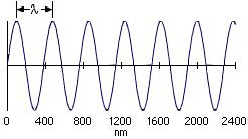
\includegraphics[width=\textwidth]{chapter7/image1}
		\caption{A picture of a wave in the ocean.}
		\label{fig:ocean-wave}
	\end{figure}
\end{minipage}\hfill%
\begin{minipage}[m]{0.45\textwidth}
	\begin{figure}[H]
		\centering
		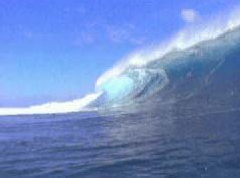
\includegraphics[width=\textwidth]{chapter7/image2}
		\caption{A wave plotted on a 2-dimensional graph.}
		\label{fig:plotted-wave}
	\end{figure}

\end{minipage}

\begin{figure}[H]
	\centering
	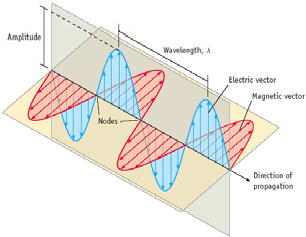
\includegraphics[width=0.75\textwidth]{chapter7/electric-magnetic-components}
	\caption{A combination of an electric component and magnetic component.}
	\label{fig:electric-magnetic-components}
\end{figure}

\section{Wavelength and Frequency}\label{sec:wavelength-and-frequency}
\begin{itemize}
	\item \definition{Wavelength}{the distance between two adjacent peaks or between two adjacent troughs.}
	\item \definition{Frequency}{the number of times per second that one complete wavelength passes a point.}
\end{itemize}

\begin{figure}[H]
	\centering
	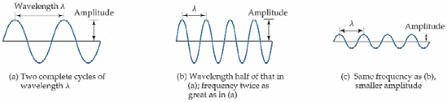
\includegraphics[width=\textwidth]{chapter7/wavelength_frequency}
	\caption{Wavelength and Frequency}
	\label{fig:wavelength-frequency}
\end{figure}

\begin{figure}[H]
	\centering
	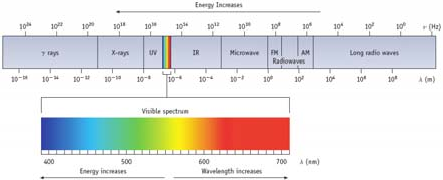
\includegraphics[width=\textwidth]{chapter7/electromagnetic-spectrum}
	\caption{Electromagnetic Spectrum}
	\label{fig:electromagnetic-spectrum}
\end{figure}

\begin{itemize}
	\item long wavelength $\epsilon \rightarrow$ small frequency
	\item short wavelength $\epsilon \rightarrow$ high frequency
	\item Therefore, wavelength and frequency are inversely related.
\end{itemize}

\section{Wavelength-Frequency Relationship}\label{sec:wavelength-frequency-relationship}
\begin{itemize}
	\item All electromagnetic radiation moves at the same speed, specifically the speed of light. $c = 2.998 \times 10^{8}$ m/s.
	\item The inverse relationship between frequency and wavelength for electromagnetic radiation is
	\begin{equation}
		\nu = \frac{c}{\lambda}
		\label{eq:wavelength-frequency-relationship}
	\end{equation}
	where $c$ is the speed of light, $\lambda$ (lambda) is the wavelength, and $\nu$ (nu) is the frequency.
\end{itemize}

%\begin{table} % FIXME: Get the wavelength table working
%	\centering
%	\caption{Common Wavelength Units}
%	\label{tab:common-wavelength-units}
%	\begin{tabular}{llll}
%		\textbf{Unit} & \textbf{Symbol} & \textbf{Length (m)} & \textbf{Type of Radiation}\\
%%		\hrule
%		Angstrom & \angstrom & $10^{-10}$ & X-ray\\
%		Nanometer & nm & $10^{-9}$ & Ultraviolet, visible\\
%		Micrometer & $\mu$m & $10^{-6}$ & Infrared\\
%		Millimeter & mm & $10^{-3}$ & Microwave\\
%		Centimeter & cm & $10^{-2}$ & Microwave\\
%		Meter & m & $1$ & TV, radio\\
%		Kilometer & km & $1000$ & Radio\\
%	\end{tabular}
%\end{table}

\section{Common Frequency Unit}\label{sec:common-frequency-unit}
\begin{itemize}
	\item Frequency is typically expressed in cycles per second, a unit also called a \emph{hertz (Hz)}. A \emph{hertz} is equivalent to reciprocal second.
	\item A particular FM radio station at a frequency of 101.3 MHz, which could also be expressed as:
	\[ 101.3 \times 10^{6} \mbox{ or } 101.3 \times 10^{6}\ s^{-1} \]
\end{itemize}

\section{Hot Objects}\label{sec:hot-objects}
\begin{itemize}
	\item Solids emit radiation when heated (referred to as \textit{Blackbody radiation}).
	\item For example, a stove burner glows bright red, while the filament in a tungsten light bulb glows white.
	\item Hotter objects glow more white.
	\item Wavelength distribution of radiation clearly depends on temperature.
\end{itemize}

\section{Quantization of Energy}\label{sec:quantization-of-energy}
\begin{itemize}
	\item An object can gain or lose enegry by absorbing or emitting radiant energy in \underline{discrete} \emph{QUANTA}.
	\item \textbf{Energy of radiation is proportional to frequency}
	\begin{equation}
		E = h \cdot \nu
		\label{eq:planck-radiation}
	\end{equation}
	where $h=6.626 \times 10^{-34} J\times s$ is Planck's constant
\end{itemize}

\section{Photoelectric Effect}\label{sec:photoelectric-effect}
\begin{itemize}
	\item Shining light on a clean metal surface causes electrons to be ejected.
	\item For example, cesium metal will emit electrons when irradiated by light with a frequency of $4.60 \times 10^{14}$ Hz or greater.
	Electrons from cesium will not be ejected if lower frequencies are used.
	\item Einstein suggested that an incident stream of tiny energy packets (quanta) were responsible for causing electrons to be ejected from the metals surface.
	\item These discrete energy packets/particles are referred to as ``photons''.
	\item Once electrons were ejected, a current could be measured.
\end{itemize}

\begin{figure}[H]
	\centering
	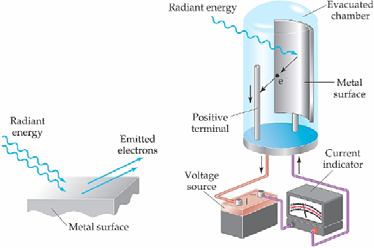
\includegraphics[width=\textwidth]{chapter7/photoelectric_effect}
	\caption{Photoelectric Effect}
	\label{fig:photoelectric-effect}
\end{figure}

\begin{itemize}
	\item Einstein was awarded the Nobel Prize in Physics in 1921 for his work on the photoelectric effect.
	\item \textbf{Energy of Photom $= E = h\nu$}, where the radiant energy is quanitzed.
	\item Radiant energy must be sufficient to overcome the attractive force between the electron and the metal itself.
	\item If an incident photon has more energy than required to remove an electron, the additional energy will be transferred to the electrons kinetic energy (i.e., energy associated with the electrons motion).
	See photoelectric worked example!
\end{itemize}

\section{Continuous Spectrum of Wavelengths from White Light}\label{sec:continuous-spectrum-of-wavelengths-from-white-light}
\begin{itemize}
	\item \definition{Continuous spectrum}{a spectrum that contains radiation distributed over all wavelengths}.
	\item In the schematic above, a white light source is used that is separated into its component colors by use of a prism.
\end{itemize}

\begin{figure}[H]
	\centering
	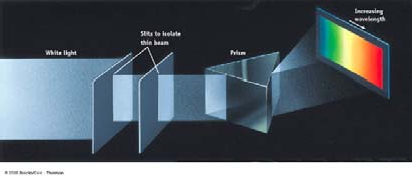
\includegraphics[width=\textwidth]{chapter7/continuous-spectrum}
	\caption{Continuous Spectrum of Wavelengths from White Light}
	\label{fig:continuous-spectrum}
\end{figure}

\section{Line Emission Spectrum of Hydrogen}\label{sec:line-emission-spectrum-of-hydrogen}
\begin{itemize}
	\item \definition{Line spectrum}{a spectrum that contains radiation at only specific wavelengths.}
	\item In the schematic above, a potential si applied to a sealed tube of hydrogen at reduced pressure.
	Passing this light through a prism results in a 4 line pattern, each with its own specific wavelength.
	The wavelengths in the hydrogen $\dots$
\end{itemize}

\begin{figure}[H]
	\centering
	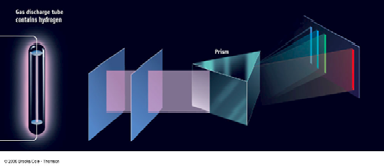
\includegraphics[width=\textwidth]{chapter7/line_emission}
	\caption{Line Emission Spectrum of Hydrogen}
	\label{fig:line-emission}
\end{figure}

\begin{figure}[H]
	\centering
	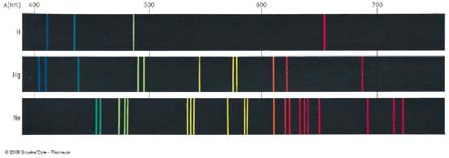
\includegraphics[width=\textwidth]{chapter7/line-emission-spectra}
	\caption{Line Emission Spectra of Hydrogen, Mercury, and Neon}
	\label{fig:line-emission-spectra}
\end{figure}

\section{Niels Bohr's Model of the Hydrogen Atom}\label{sec:niels-bohr's-model-of-the-hydrogen-atom}
Model based on the following three postulates
\begin{itemize}
	\item Only orbits of certain radii, corresponding to certain definite energies, are permitted for the electron in the hydrogen atom.
	\item An electron in a permitted orbit has a specific energy and is in an ``allowed'' energy state.
	An electron in an allowed energy state will not radiate energy and therefore will not spiral into the nucleus.
	\item Energy is emitted or absorbed by the electron only as the electron changes from one allowed energy state to another.
	(This energy is emitted or absorbed as a \emph{photon}~\eqref{eq:planck-radiation})
\end{itemize}

\section{The Energy States of the Hydrogen Atom}\label{sec:the-energy-states-of-the-hydrogen-atom}
\begin{minipage}[m]{0.45\textwidth}
	\begin{figure}[H]
		\centering
		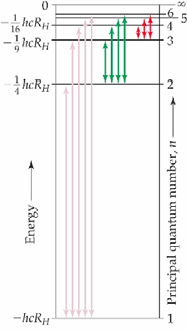
\includegraphics[width=\textwidth]{chapter7/image16}
		\caption{The Energy States of the Hydrogen Atom}
		\label{fig:hydrogen-atom-energy-states}
	\end{figure}
\end{minipage}\hfill%
\begin{minipage}[m]{0.45\textwidth}
	\begin{equation}
		\begin{aligned}
			E_{n} &= -hcR_{H}\left( \frac{1}{n^{2}} \right)\\
			&= -2.18 \times 10^{-18} J\ \left( \frac{1}{n^{2}} \right)
		\end{aligned}
		\label{eq:bohr-energy-state}
	\end{equation}
	\begin{itemize}
		\item $h$, $c$ and $R_{H}$ are Planck's constant, the speed of light, and Rydberg's constant, respectively.
		\item $n$ is called the \emph{principal quantum number}, and takes on whole integer values in $[1, \infty)$.
		\item The lowest energy state $(n=1)$ is called the \emph{ground state.}
		\item When an electron occupies the $n=2$ orbit or higher, the atom is said to be in an \emph{excited state}.
	\end{itemize}
\end{minipage}

\section{Electronic Transitions in the Hydrogen Atom}\label{sec:electronic-transitions-in-the-hydrogen-atom}
\begin{itemize}
	\item An electron can move to a higher energy state if energy is absorbed.
	\item Conversely, radiant energy is emitted when the electron falls to a lower energy state.
\end{itemize}

\begin{figure}[H]
	\centering
	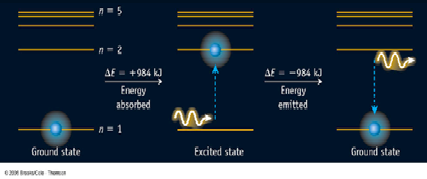
\includegraphics[width=\textwidth]{chapter7/electron_transitions}
	\caption{Electron Transitions in the Hydrogen Atom}
	\label{fig:electron-transitions}
\end{figure}

\begin{figure}[H]
	\centering
	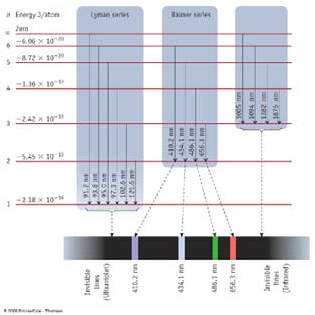
\includegraphics[width=\textwidth]{chapter7/paschen_series}
	\caption{Paschen Series}
	\label{fig:paschen-series}
\end{figure}

\begin{itemize}
	\item Notice that the energy is lowest (most negative) for $n = 1$.
	\item The energy difference between the \textit{final} and \emph{initial} states is given by the \emph{following equation:}
	\begin{equation}
		\begin{aligned}
			\Delta E &= E_{final} - E_{initial}\\
			&= E_{photon}\\
			&= h\nu
		\end{aligned}
		\label{eq:electronic-transition-difference}
	\end{equation}
	\item Substituting~\eqref{eq:bohr-energy-state} into the above equation, while taking into account that $\nu = c / \lambda$, the following results:
	\begin{equation}
		\begin{aligned}
			\Delta E &= h\nu\\
			&= \frac{hc}{\lambda}\\
			&= -2.18 \times 10^{-18} J\ \left( \frac{1}{n_{f}^{2}} - \frac{1}{n_{i}^{2}} \right)\\
			&= 2.18 \times 10^{-18} J\ \left( \frac{1}{n_{i}^{2}} - \frac{1}{n_{f}^{2}} \right)
		\end{aligned}
		\label{eq:electron-transition}
	\end{equation}
	\item Another useful equation for directly calculating wavelength is as follows:
	\[ \frac{1}{\lambda} = R_{H}\left( \frac{1}{n_{i}^{2}} - \frac{1}{n_{f}^{2}} \right) \]
\end{itemize}

\section{The Wave Behavior of Matter}\label{sec:the-wave-behavior-of-matter}
\begin{itemize}
	\item Louis de Broglie (1892-1987) suggested that a stream of particles should also exhibit properties of a wave.
	\item He proposed that the characteristic wavelength of a particle (e.g., an electron) depends on its mass $(m)$ and velocity $(v)$.
	The quantity $mv$ is the \emph{momentum} and $h$ is simply Planck's constant.
	\begin{equation}
		\lambda = \frac{h}{mv}
		\label{eq:wave-behavior-of-matter}
	\end{equation}
	\item The equation provides sufficient wavelengths for particles of small mass (e.g., an electron) but not for ones for large mass.
	Due to the inverse relationship, as the mass gets very large, the corresponding wavelength becomes small and thus difficult to observe experimentally.
\end{itemize}

\section{Heisenberg's Uncertainty Principle}\label{sec:heisenberg's-uncertainty-principle}
\begin{itemize}
	\item Werner Heisenberg (1901-1976).
	The \emph{Heisenberg uncertainty principle} states that there is an inherent uncertainty in the precision with which we can simultaneously specify the position and momentum of extremely small particles, such as an electron.
	\item Mathematically:
	\begin{equation}
		\Delta x \cdot \Delta (mv) \geq \frac{h}{2\pi}
		\label{eq:heisenberg-uncertainty-principle}
	\end{equation}
	\item where $\Delta x$ is the uncertainty in the particle's position and $\Delta (mv)$ is the uncertainty in its momentum.
\end{itemize}

\section{Quantum Mechanics and Atomic Orbitals}\label{sec:quantum-mechanics-and-atomic-orbitals}
\begin{itemize}
	\item Erwin Schr{\:o}dinger (1887-1961), an Austrian physicist, developed an equation to describe both the wave- and particle-like behavior of the electron.
	\item Requires the use of complex calculus.
	\item Solving the Schr{\:o}dinger equation provides a series of mathematical functions called \emph{wave functions} that describe the electron in an atom.
	\item The wave functions are denoted by the lowercase Greek letter \emph{$\psi$} (psi).
	\item \emph{$\psi^{2}$} is the probability or electron density.
	It relates to the probability of finding an electron in a certain region of space at a given instant.
\end{itemize}

\section{Electron-Density Distribution in a Hydrogen Atom}\label{sec:electron-density-distribution-in-a-hydrogen-atom}
\begin{itemize}
	\item Diagram represents the probability of finding an electron in the ground state of a hydrogen atom.
\end{itemize}
\begin{figure}[H]
	\centering
	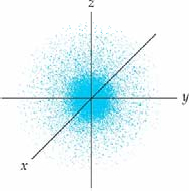
\includegraphics[width=0.5\textwidth]{chapter7/electron_density_distribution}
	\caption{Electron-Density Distribution in a Hydrogen Atom}
	\label{fig:electron-density-distribution}
\end{figure}

\section{Orbitals and Quantum Numbers}\label{sec:orbitals-and-quantum-numbers}
\begin{itemize}
	\item The wave function $\psi$ depends on four quantum numbers ($n$, $l$, $m_{l}$, and $m_{s}$)
	\begin{description}[font=\emph]
		\item[Principal quantum number $n$] that can have integral values of 1, 2, 3, $\dots$.
		As $n$ increases, the orbital becomes larger and the electron is further from the nucleus.
		\item[Angular momentum quantum number $l$] can take on integral values from 0 to $n-1$ for each defined value of $n$.
		\item[Magnetic quantum number $m_{l}$] that can take values of $-l$ to $+l$, including 0.
		\item[Spin magnetic quantum number $m_{s}$] are two possible values are $+\frac{1}{2}$ (spin pointing up) and $-\frac{1}{2}$ (spin pointing down).
	\end{description}
\end{itemize}

\section{Shells and Subshells}\label{sec:shells-and-subshells}
\begin{description}[font=\emph]
	\item[Electron Shell] A collection of orbitals with the same value of $n$.
	\item[Subshell] A set of orbitals that have the same $n$ and $l$ values.
\end{description}

%\begin{table}[H] % FIXME: This table is also messed up
%	\centering
%	\caption{Value of $l$ and Corresponding Letter Designation}
%	\label{tab:l-letter-designations}
%	\begin{tabular}{cc}
%		\textbf{Value of $l$} & \textbf{Corresponding Subshell Label}\\
%		0 & $s$\\
%		1 & $p$\\
%		2 & $d$\\
%		3 & $f$\\
%	\end{tabular}
%\end{table}

%\begin{table}[H] % FIXME: This table too
%	\centering
%	\caption{Number of Orbitals in a Subshell}
%	\label{tab:subshell-orbitals}
%	\begin{tabular}{cc}
%		\textbf{Value of $l$} & \textbf{Corresponding Subshell Label}\\
%		0 & $s$\\
%		1 & $p$\\
%		2 & $d$\\
%		3 & $f$\\
%	\end{tabular}
%\end{table}

\section{Electron Configurations}\label{sec:electron-configurations}
\begin{itemize}
	\item We use the \emph{Aufbau Principle} for filling electrons from bottom to top.
	\item \definition{Pauli Exclusion Principle}{a maximum of two electrons can be placed in an orbital and must have opposite spin.}
	\item \definition{Hunds Rule}{for degenerate orbitals, the lowest energy is attained when the number of electrons with the same spin is maximized.}
\end{itemize}

\end{document}
